\usetikzlibrary{arrows.meta,decorations.pathmorphing,fadings}

\begin{frame}[fragile,label=typicalPatternSnake]{typical pattern}
\begin{tikzpicture}
\tikzset{
    thread/.style={very thick,draw,decorate,decoration=snake},
    split/.style={very thick,draw},
    marker/.style={thin,draw},
}
\path[thread] (0, 0) --  (0, -.5);
\node[anchor=south] at (0,0) {parent};
\node[anchor=north] (fork mark) at (0, -.5) {fork};
\draw[thread] (fork mark.south) -- (0, -2) node[below] (wait start) {waitpid};
\node (child start) at (9, -1.5) {child process};
\path[split] (fork mark) --  (child start);
\path[thread] (child start.south) -- (9, -2.5) node[below] (exec) {exec};
\path[thread] (exec.south) -- ++(0, -2) coordinate (exec done);
\path[marker] (exec done) -- ++(.5, 0) node[right] {exit()};
\path[split,dotted] (exec done) -- (0, -6);
\draw[very thick,dashed] (wait start) -- (0, -6);
\path[thread] (0, -6) -- ++(0, -3);
\end{tikzpicture}
\end{frame}


\begin{frame}[fragile,label=typicalPatternSnakeAlt]{typical pattern (alt)}
\begin{tikzpicture}
\tikzset{
    thread/.style={very thick,draw,decorate,decoration=snake},
    split/.style={very thick,draw},
    marker/.style={thin,draw},
}
\path[thread] (0, 0) --  (0, -.5);
\node[anchor=south] at (0,0) {parent};
\node[anchor=north] (fork mark) at (0, -.5) {fork};
\draw[thread] (fork mark.south) -- (0, -5.5) node[below] (wait start) {waitpid};
\node (child start) at (9, -1.5) {child process};
\path[split] (fork mark) --  (child start);
\path[thread] (child start.south) -- (9, -2.5) node[below] (exec) {exec};
\path[thread] (exec.south) -- ++(0, -1) coordinate (exec done);
\path[marker] (exec done) -- ++(.5, 0) node[right] {exit()};
\path[split,dotted] (exec done) -- (wait start.east);
%\draw[very thick,dashed] (wait start) -- (0, -6);
\path[thread] (wait start.south) -- ++(0, -3);
\end{tikzpicture}
\end{frame}

\begin{frame}[fragile,label=typicalPattern]{typical pattern (detail)}
\newcommand{\maincode}{
            pid = fork(); \\
            if (pid == 0) \{ \\
            \hspace{.5cm} exec\ldots(\ldots); \\
            \hspace{.5cm} \ldots \\
            \} else if (pid > 0) \{ \\
            \hspace{.5cm} waitpid(pid,\ldots); \\
            \hspace{.5cm} \ldots \\
            \} \\
            \ldots 
}
\newcommand{\maincodeExec}{
            pid = fork(); \\
            if (pid == 0) \{ \\
            \hspace{.5cm} \myemph{exec\ldots(\ldots);} \\
            \hspace{.5cm} \ldots \\
            \} else if (pid > 0) \{ \\
            \hspace{.5cm} waitpid(pid,\ldots); \\
            \hspace{.5cm} \ldots \\
            \} \\
            \ldots 
}
\newcommand{\maincodeWait}{
            pid = fork(); \\
            if (pid == 0) \{ \\
            \hspace{.5cm} exec\ldots(\ldots); \\
            \hspace{.5cm} \ldots \\
            \} else if (pid > 0) \{ \\
            \hspace{.5cm} \myemph{waitpid(pid,\ldots);} \\
            \hspace{.5cm} \ldots \\
            \} \\
            \ldots 
}
\newcommand{\altcode}{
            main() \{ \\
            \hspace{.5cm} \ldots \\
            \} \\
}
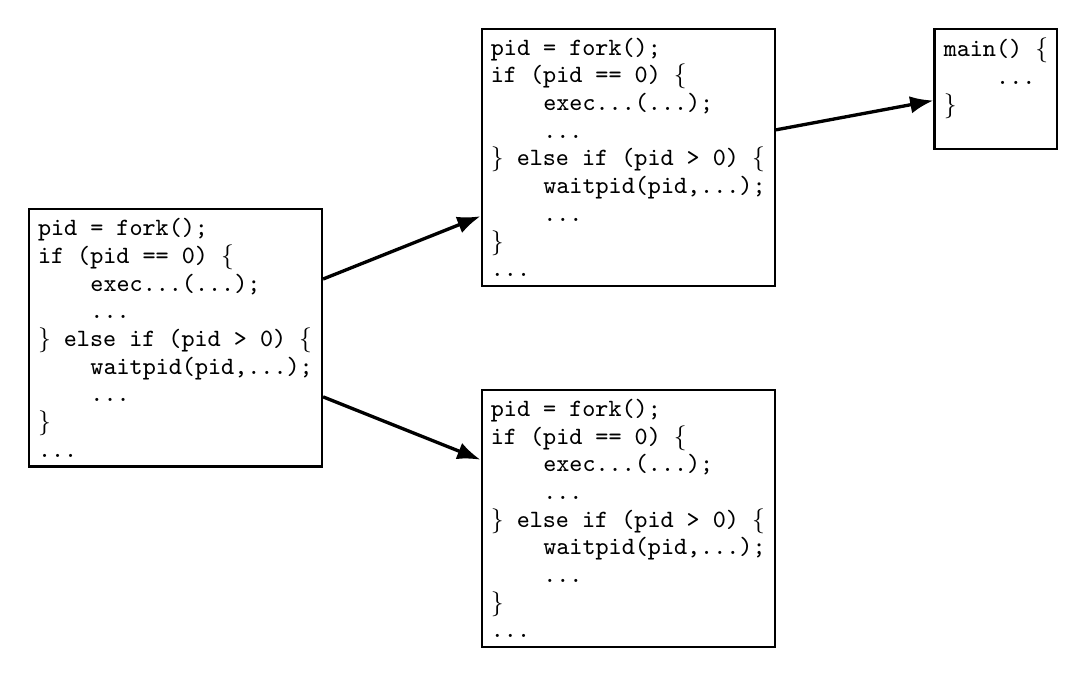
\begin{tikzpicture}
\tikzset{
    code box/.style={draw,thick,font=\tt\fontsize{9}{10}\selectfont,align=left},
    with the code/.style={
        code box,
    },
    with the other code/.style={
        code box,
    }
}
\node[with the code] (start) {\maincode};
\node[with the code,anchor=north west] (parent first) at ([xshift=2cm,yshift=1cm]start.south east) {\maincodeWait};
\node[with the code,anchor=south west] (child first) at ([xshift=2cm,yshift=-1cm]start.north east) {\maincodeExec};
\node[with the other code,anchor=north west] (child second) at ([xshift=2cm]child first.north east) {\altcode};

\begin{scope}[very thick,>=Latex]
\draw[->] (start) -- (parent first);
\draw[->] (start) -- (child first);
\draw[->] (child first) -- (child second);
\end{scope}
\end{tikzpicture}
\end{frame}

